\section{Plugin Catalog}
\label{sec:chapter_3_section_4}

\noindent
It is pivotal to provide the system users with a rich catalog of plugins, to cover all the basic as well as the most advanced modeling requirements.
Table~\ref{tab:plugins-example} (see Figure~\ref{fig:catalog}) reports examples of plugins arranged according to the  taxonomy introduced in Section~\ref{ssec:taxonomy}.

\begin{figure}[htbp] %  figure placement: here, top, bottom, or page
   \centering
   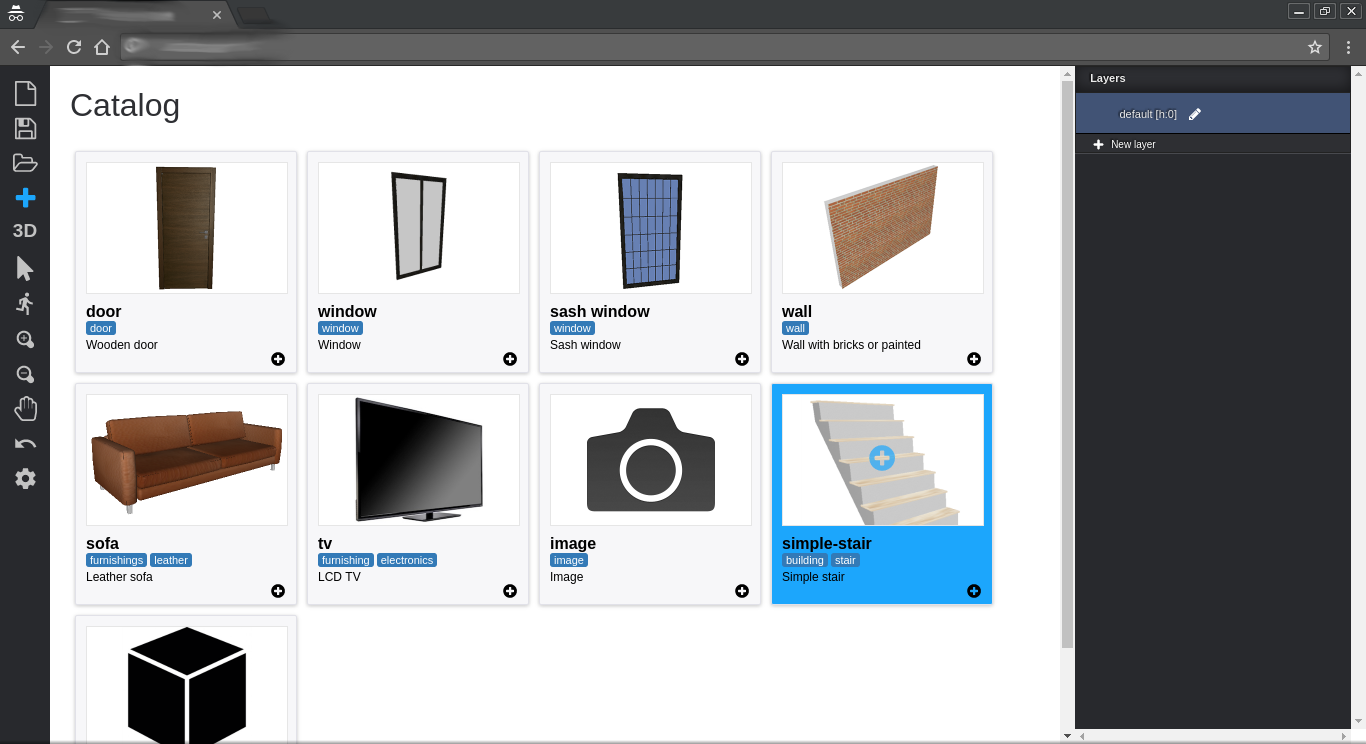
\includegraphics[width=1\linewidth]{images/figcatalog}
   \caption{Catalogo dei Plugins}
   \label{fig:catalog}
\end{figure}
